\graphicspath{ {../images/} } 

Wir betrachten die Hisense EN2A27 Fernbedienung. 

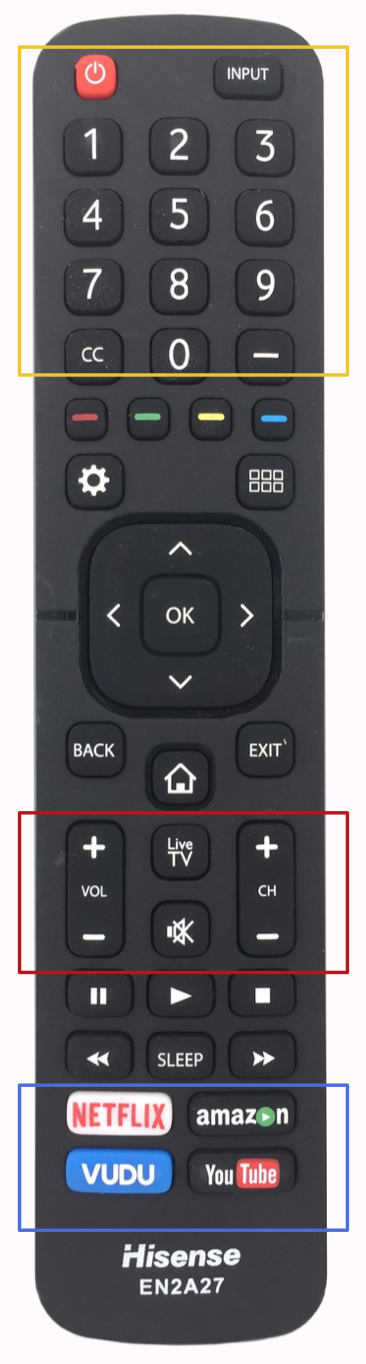
\includegraphics[scale=.5]{remote}

\begin{itemize}
  \item Gelb markiert sehen wir eine sequentielle Anordnung: Oft nach dem Einschalten des
        Fernsehrs muss man zu einem Sender oder Input-Kanal wechseln.
  \item Rot markiert sehen wir eine funktionalle Anordnung: Den Kanal oder die
    Lautstärke zu verändern erfolgt nach dem selben "'Hoch"'-"'Runter"' Prinzip
    und ist deshalb gemeinsam angeordnet
  \item Blau markiert sehen wir eine Anordnung gemäss Häufigkeit: Der Benutzer
    startet oft verwendetet Streaming-Dienste direkt über dedizierte Buttons
\end{itemize}
